\documentclass{article}
\usepackage{graphicx,amsmath,amssymb,float} % Required for inserting images

\title{CP_Ps4}

\date{October 2023}

\begin{document}



\section{Problem 1}
The approximate error leaves neglects errors of $\mathcal{O}\left(h^3\right)$ or higher in approximating the true error so it will be off. The approx error is  0.026633333333333137 and the real error is 0.026660000000000572
\section{Problem 2}
\subsection{a}\begin{align*}
    &E=\frac{m}{2}\frac{dq}{dt}^2+V(q)\\
    &\frac{2}{m}\left(E-V(q)\right)=\frac{dq}{dt}^2\\
    &dt=\sqrt{\frac{m}{2}}\frac{dq}{\sqrt{E-V(q)}}\\
    &t |^{t=T/4}_{0}=\int_0^a\sqrt{\frac{m}{2}}\frac{dq}{\sqrt{E-V(q)}}\\
    &\frac{T}{4}=\int_0^a\sqrt{\frac{m}{2}}\frac{dq}{\sqrt{E-V(q)}}\\
    &T=\sqrt{8m}\int_0^a\frac{dq}{\sqrt{E-V(q)}}\\
\end{align*}
\subsection{b} 
\begin{figure}[H]
    \centering
    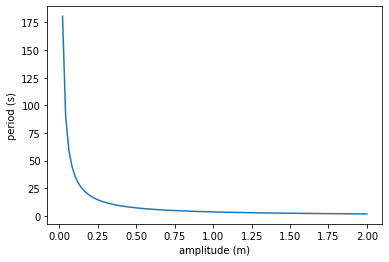
\includegraphics[width=\textwidth]{plot 5.10b.png}
    \caption{Period of Oscillator against amplitude}
    \label{fig:enter-label}
\end{figure}
\subsection{c}
As $a\rightarrow 0$, the physical situation becomes a particle at rest in equilibrium. This particle wont move thus an infinite period. For potential that goes as $x^n$ the integral can be approximated as $\approx \frac{a}{\sqrt{a^n}}$. Thus for $n<2$, the period increases as $a$ grows, vice versa for $n>2$. At $n=2$, we expect a constant period for any initial amplitude, which is what we see for a simple harmonic oscillator.
\section{Problem 3}
  
Notice for this problem $\left [\sqrt{\frac{m\omega}{\hbar}}   \right] = \frac{1}{L}$ is unitless. Therefor, distance is unitless. Amplitude needs unit such that when square and integrated over distance, it gives a unitless probability. Therefor amplitude is also unitless here.
For Hermite-Gaussian quadrature to perfectly determine the rms distance of a wave function of energy $n$, it needs $2n+2$ points, $2n$ for the $n^2$ of the wave-function square amplitude, plus 2 from the $x^2$ term.

\begin{figure}
    \centering
    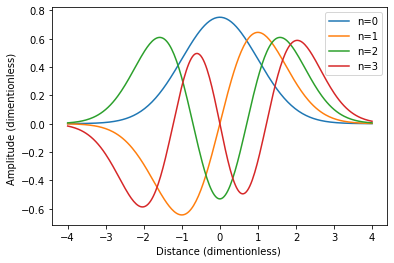
\includegraphics[width=\textwidth]{10.16a.png}
    \caption{$|0\rangle$,$|1\rangle$,$|2\rangle$,$|3\rangle$}
    \label{fig:enter-label}
\end{figure}
\begin{figure}
    \centering
    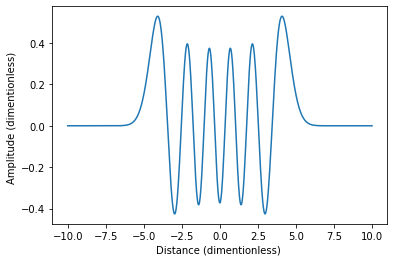
\includegraphics[width=\textwidth]{10.16b.png}
    \caption{$|10\rangle$}
    \label{fig:enter-label}
\end{figure}
\end{document}
